\documentclass[10pt]{beamer}

\usetheme[progressbar=frametitle]{metropolis}

\usepackage{booktabs}
\usepackage[scale=2]{ccicons}

\usepackage{minted}
\newminted{haskell}{tabsize=4}
\usemintedstyle{trac}

\usepackage{pgf}
\usepackage{tikz}
\usetikzlibrary{arrows,automata}

\usepackage{amsmath}

\usepackage{pgfplots}
\usepgfplotslibrary{dateplot}

\usepackage{xspace}
\newcommand{\themename}{\textbf{\textsc{metropolis}}\xspace}

\title{Ragax: Ragalur Expressions}
\subtitle{Using derivatives to validate Indian Classical Music}
\date{27 April 2016}
\author{Walter Schulze}
\institute{Cape Town Functional Programming Meetup}

\usepackage{xcolor}
\def\valid{${\color{mLightGreen} \checkmark}$}
\def\invalid{{\color{mLightBrown} x}}

\begin{document}

\maketitle

\begin{frame}{Key Takeaways}
After this talk you should be able to:
\begin{itemize}
\item implement a regular expression matcher function and
\item invent your own regular expression operators,
\end{itemize}
because \textbf{derivatives are that simple}.

You will also learn about:
\begin{itemize}
\item the most basic concept of a Raga;
\item laziness, memoization and least fixed point;
\item derivatives for context free grammars; and
\item derivatives for trees.
\end{itemize}
\end{frame}

\section{Regular Expressions}

\begin{frame}[fragile]{Matching a string of characters}
Using a regex we can validate a string.
$$
a(a|b)*
$$
\begin{center}
\begin{tabular}{ll}
ab & \valid \\
aabbba & \valid \\
ac & \invalid \\
ba & \invalid \\
\end{tabular}
\end{center}
$$
a \cdot (a\ |\ b)^{*}
$$
\end{frame}

\section{Derivatives}

\begin{frame}{Easy}
The Brzozowski derivative is the \textbf{easiest way to evaluate a regular expression}.

Three functions:
\begin{itemize}
\item Nullable
\item Simplification (optional)
\item Derivative
\end{itemize}
\end{frame}


\begin{frame}{What is a Derivative}
The derivative of an expression is the expression that is left to match after the given character has been matched
\cite{brzozowski1964derivatives}.

For example:

\begin{center}
\begin{tabular}{lll}
$\partial_a a \cdot b \cdot c$ & = & $b \cdot c$ \\
$\partial_a (a \cdot b\ |\ a \cdot c)$ & = & $(b\ |\ c)$ \\
$\partial_b b \cdot c$ & = & $c$ \\
$\partial_c c$ & = & $\epsilon$ \\
$\partial_a a^{*}$ & = & $a^{*}$ \\
\end{tabular}
\end{center}

\end{frame}

\begin{frame}{Basic Operators}
\begin{center}
\begin{tabular}{l|r}
empty set & $\emptyset$ \\
empty string & $\varepsilon$ \\
character & $a$ \\
concatenation & $r \cdot s$ \\
zero or more & $r^*$ \\
logical or & $r\ |\ s$ \\
\end{tabular}
\end{center}
\end{frame}

\begin{frame}[fragile]
\frametitle{Basic Operators}
\begin{center}
\begin{minted}{haskell}
data Regex = EmptySet
  | EmptyString
  | Character Char
  | Concat Regex Regex
  | ZeroOrMore Regex
  | Or Regex Regex
\end{minted}
\end{center}
\end{frame}

\begin{frame}[fragile]{Nullable}
Does the expression match the empty string.
\begin{center}
\begin{tabular}{l c l}
$\nu(\emptyset)$ & = & false\\
$\nu(\varepsilon)$ & = & true\\
$\nu(a)$ & = & false\\
$\nu(r \cdot s)$ & = & $\nu(r)\ and\ \nu(s)$ \\
$\nu(r^{*})$ & = & true \\
$\nu(r\ |\ s)$ & = & $\nu(r)\ or\ \nu(s)$ \\
\end{tabular}
\end{center}
\end{frame}

\begin{frame}[fragile]{Nullable}
Does the expression match the empty string.
\begin{center}
\begin{minted}{haskell}
nullable :: Regex -> Bool
nullable EmptySet = False
nullable EmptyString = True
nullable (Character _) = False
nullable (Concat a b) = nullable a && nullable b
nullable (ZeroOrMore _) = True
nullable (Or a b) = nullable a || nullable b
\end{minted}
\end{center}
\end{frame}

\begin{frame}{Nullable Examples}
\begin{center}
\begin{tabular}{l c l}
$\nu(a \cdot b \cdot c)$ & = & $\invalid$ \\
$\nu(\varepsilon)$ & = & $\valid$ \\
$\nu(a\ |\ b)$ & = & $\invalid$\\
$\nu(\varepsilon\ |\ a)$ & = & $\valid$\\
$\nu(a \cdot \varepsilon)$ & = & $\invalid$ \\
$\nu((a \cdot b)^{*})$ & = & $\valid$ \\
$\nu(c \cdot (a \cdot b)^{*})$ & = & $\invalid$ \\
\end{tabular}
\end{center}
\end{frame}

\begin{frame}{Derivative Rules}
\begin{center}
\begin{tabular}{l c l}
$\partial_a \emptyset$ & = & $\emptyset$ \\
$\partial_a \epsilon$ & = & $\emptyset$ \\
$\partial_a a$ & = & $\epsilon$ \\
$\partial_a b$ & = & $\emptyset \ \ $ for $b \ne a$ \\
$\partial_a (r \cdot s) $ & = & $\partial_a r \cdot s\ |\  \jmath(r) \cdot \partial_a s $ \\
$\partial_a (r^{*}) $ & = & $\partial_a r \cdot r^{*} $ \\
$\partial_a (r\ |\ s) $ & = & $\partial_a r\ |\ \partial_a s $ \\
\end{tabular}
\end{center}

\begin{center}
\begin{tabular}{l c l r}
$\jmath(r)$ & = & $\epsilon$ & if $\nu(r)$ \\
 & = & $\emptyset$ & otherwise \\
\end{tabular}
\end{center}
\end{frame}

\begin{frame}[fragile]{Derivative Rules}
\begin{center}
\begin{haskellcode}
deriv :: Expr -> Char -> Expr
deriv EmptyString c = EmptySet
deriv EmptySet c = EmptySet
deriv (Character a) c = if a == c 
  then EmptyString else EmptySet
deriv (Concat r s) c =
  let left = deriv r c
      right = deriv s c
  in if nullable r
     then Or (Concat left s) right
     else Concat left s
deriv (ZeroOrMore r) c =
  Concat (deriv r c) (ZeroOrMore r)
deriv (Or r s) c =
  Or (deriv r c) (deriv s c)
\end{haskellcode}
\end{center}
\end{frame}

\begin{frame}[fragile]{Simplification}
\begin{center}
\begin{tabular}{lll}
$\emptyset \cdot r$ & $\approx$ & $\emptyset$ \\
$r \cdot \emptyset$ & $\approx$ & $\emptyset$ \\
$\varepsilon \cdot r$ & $\approx$ & $r$ \\
$r \cdot \varepsilon$ & $\approx$ & $r$ \\
\\
$r\ |\ r$ & $\approx$ & $r$ \\
$\emptyset\ |\ r$ & $\approx$ & $r$ \\
\\
$(r^{*})^{*}$ & $\approx$ & $r^{*}$ \\
$\varepsilon^{*}$ & $\approx$ & $\varepsilon$ \\
$\emptyset^{*}$ & $\approx$ & $\varepsilon$ \\
\end{tabular}
\end{center}
\end{frame}

\begin{frame}[fragile]{Execution}
$$
\nu(foldl(\partial, r, str))
$$
$$
\nu(foldl(simp \cdot \partial, r, str))
$$
\begin{center}
\begin{haskellcode}
nullable $ foldl (simplify . deriv) expr string
\end{haskellcode}
\end{center}
\begin{center}
\begin{minted}{go}
func matches(r *expr, str string) bool {
    for _, c := range str {
        r = simplify(deriv(r, c))
    }
    return nullable(r)
}
\end{minted}
\end{center}
\end{frame}

\begin{frame}[fragile]{Example: Matching a sequence of notes}
Using a regex we can validate the C Major Pentatonic Scale.
$$
c\cdot(c|d|e|g|a)^{*}
$$
\begin{center}
\begin{tabular}{ll}
ceg & \valid \\
\end{tabular}
\end{center}

\begin{center}
\begin{tabular}{llr}
$\partial_c c\cdot(c|d|e|g|a)^{*}$ & = & $\varepsilon \cdot (c|d|e|g|a)^{*}$\\
$\partial_e \varepsilon \cdot (c|d|e|g|a)^{*}$ & = & 
$(\emptyset \cdot (c|d|e|g|a)^{*})\ |\ (\emptyset | \emptyset | \varepsilon | \emptyset | \emptyset) \cdot (c|d|e|g|a)^{*}$ \\
& = & $(c|d|e|g|a)^{*}$\\
$\partial_g (c|d|e|g|a)^{*}$ & = & $(\emptyset | \emptyset | \emptyset | \varepsilon | \emptyset) \cdot (c|d|e|g|a)^{*}$\\
& = & $(c|d|e|g|a)^{*}$\\
\end{tabular}
\end{center}
\begin{center}
$\nu((c|d|e|g|a)^{*})$ = \valid
\end{center}
\end{frame}

\plain{Questions?}

\begin{frame}[fragile]{Deterministic Finite Automata}
$$
c\cdot(c|d|e|g|a)^{*}
$$
\begin{center}
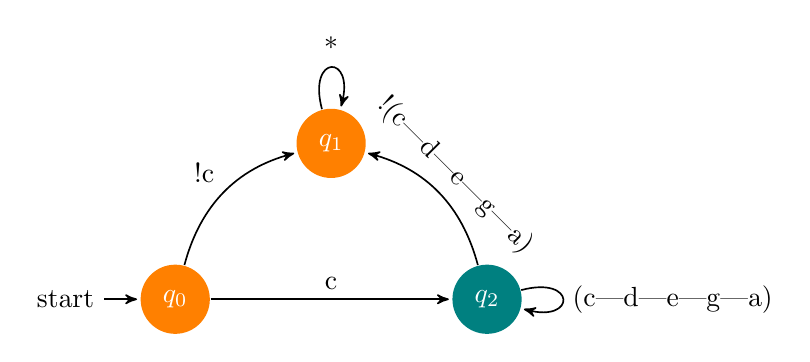
\begin{tikzpicture}[->,>=stealth',shorten >=1pt,auto,node distance=2.8cm,semithick]
  \tikzstyle{every state}=[fill=orange,draw=none,text=white]

  \node[initial,state] (A)                    {$q_0$};
  \node[state]         (B) [above right of=A] {$q_1$};
  \node[state,fill=teal]         (C) [below right of=B] {$q_2$};

  \path (A) edge [bend left]  node {!c} (B)
            edge              node {c} (C)
        (B) edge [loop above] node {*} (B)
        (C) edge [bend right] node [sloped, above] {!(c|d|e|g|a)} (B)
        (C) edge [loop right] node {(c|d|e|g|a)}  (C);
\end{tikzpicture}
\end{center}
\end{frame}

\begin{frame}[fragile]{Memoization and Simplification}
\begin{center}
\begin{tabular}{lll}
$q_0$ & = & $c\cdot(c|d|e|g|a)^{*}$ \\
$q_1$ & = & $\emptyset$ \\
$q_2$ & = & $(c|d|e|g|a)^{*}$ \\
\end{tabular}
\end{center}
\begin{center}
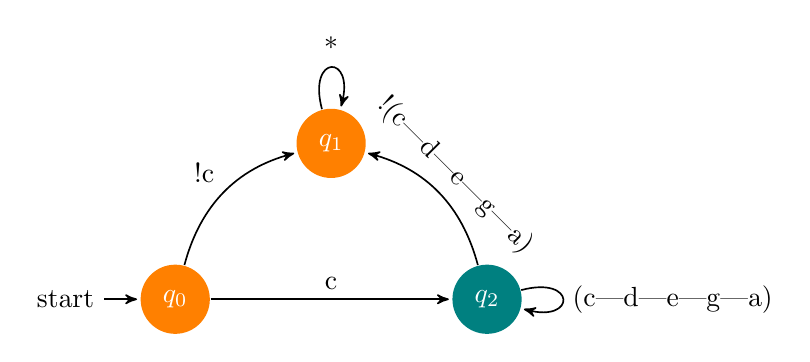
\begin{tikzpicture}[->,>=stealth',shorten >=1pt,auto,node distance=2.8cm,semithick]
  \tikzstyle{every state}=[fill=orange,draw=none,text=white]

  \node[initial,state] (A)                    {$q_0$};
  \node[state]         (B) [above right of=A] {$q_1$};
  \node[state,fill=teal]         (C) [below right of=B] {$q_2$};

  \path (A) edge [bend left]  node {!c} (B)
            edge              node {c} (C)
        (B) edge [loop above] node {*} (B)
        (C) edge [bend right] node [sloped, above] {!(c|d|e|g|a)} (B)
        (C) edge [loop right] node {(c|d|e|g|a)}  (C);
\end{tikzpicture}
\end{center}
\begin{itemize}
\item Memoizing deriv = transition function
\item Memoizing nullable = accept function
\item Simplification = minimization \cite{owens2009regular}
\end{itemize}
\end{frame}

\section{Ragas - Indian Classical Music \\ \\
Thank you:\\ Ryan Lemmer\\ Antoine Van Gelder}

\plain{Video https://www.youtube.com/watch?v=iElMWziZ62A}

\begin{frame}{Ragas}
\begin{itemize}
\item Ragas are indian version of western scales \cite{Raga2011}.
\item Stricter than western scales.
\item Possible next note depends on current note.
\item Notes labeled differently and relative to root note.
\end{itemize}
\begin{center}
\begin{tabular}{l|llllllllllll}
Raga & S & r & R & g & G & m & M & P & d & D & n & N \\
Western & c & c$\sharp$ & d & d$\sharp$ & e & f & f$\sharp$ & g & g$\sharp$ & a & a$\sharp$ & b \\
\end{tabular}
\end{center}
I will skip over microtones and all the other theory, just because its not relevant to this talk.
\end{frame}

\begin{frame}{Example Raga}
\begin{itemize}
\item Raag Bhupali (a type of Pentatonic scale)
\item Ascent: S R G P D S'
\item Descent: S' D P G R S
\end{itemize}
\begin{itemize}
\item Western Pentatonic scale
\item Ascent: c d e g a c$^{1}$
\item Descent: c$^{1}$ a g e d c
\end{itemize}

Given the current note you must choose the next ascending or descending note.

For example given G (e) you can choose P (g) if you want to ascend or R (d) if you want to descend.
\end{frame}

\plain{Play Raag Bhupali}
% http://raag-hindustani.com/22_files/ArohBhupali.mp3

\plain{Questions?}

\section{An expression for a Raga}

\begin{frame}{Recursive Regular Expressions}
\begin{itemize}
\item One extra concept: Reference
\item Two operations
\item Define a reference: $\#myref = (a \cdot b)^{*}$
\item Use a reference: $(@myref\ |\ c)$
\end{itemize}
\begin{center}
\begin{tabular}{l c l}
$\partial_a @q$ & = & $\partial_a \#q$ \\
$\nu(@q)$ & = & $\nu(\#q)$ \\
\end{tabular}
\end{center}
\end{frame}

\begin{frame}{A Grammar for a Raga}
\begin{itemize}
\item Raag Bhupali (a type of Pentatonic scale)
\item Ascent: S R G P D S'
\item Descent: S' D P G R S
\end{itemize}
\begin{center}
\begin{tabular}{lll}
$\#S$ & = & $(S \cdot ( @R\ |\ @D ))^{*}$ \\
$\#R$ & = & $R \cdot ( @G\ |\ \varepsilon )$ \\
$\#G$ & = & $G \cdot ( @P\ |\ @R )$ \\
$\#P$ & = & $P \cdot ( @D\ |\ @G )$ \\
$\#D$ & = & $D \cdot ( \varepsilon\ |\ @P )$ \\
\end{tabular}
\end{center}
\end{frame}

\plain{Demo}

\section{Context Free Grammars}

\begin{frame}{Left Recursive Raga}
\begin{center}
\begin{tabular}{lllll}
$\#S$ & {\color{gray}=} & {\color{gray} $(S \cdot ( @R\ |\ @D ))^{*}$} & = & $@S \cdot (S \cdot ( @R\ |\ @D ))\ |\ \varepsilon$ \\
$\#R$ & = & $R \cdot ( @G\ |\ \varepsilon )$ \\
$\#G$ & = & $G \cdot ( @P\ |\ @R )$ \\
$\#P$ & = & $P \cdot ( @D\ |\ @G )$ \\
$\#D$ & = & $D \cdot ( \varepsilon\ |\ @P )$ \\
\end{tabular}
\end{center}


nullable and derivative each have infinite recursion.
$$
\nu(\#S) = (\nu(@S)\ and\ \nu(S \cdot ( @R\ |\ @D )))\ or\  \nu(\varepsilon)
$$
\end{frame}

\begin{frame}{Parsing with Derivatives}
This has been solved using \cite{might2011parsing} functional concepts:
\begin{itemize}
\item laziness - The Brake
\item memoization - The Handbrake
\item least fixed point - The Gas
\end{itemize}
\end{frame}

\begin{frame}[fragile]{Laziness}
Instead of evaluating a function and returning a value, 
\begin{minted}{go}
func eval(params ...) value {
    ...
    return value(...)
}
\end{minted}
we defer the evaluation and return a function that will return the value.
\begin{minted}{go}
func lazyEval(params ...) func() value {
    return func() value {
        return eval(params)
    }
}
\end{minted}
\end{frame}

\begin{frame}{Memoization}
\begin{center}
A function's results are cached for the given inputs.
\end{center}
\end{frame}

\begin{frame}[fragile]{Least Fixed Point}
\begin{center}
When a function call results in calling the same function with the same inputs, we return a chosen fixed point.
\end{center}
\end{frame}

\begin{frame}{Laziness - The Brake}
Instead of storing the field values of \textbf{concat}, \textbf{or} and \textbf{zero or more} we rather store functions that when called will return the value of the field.

This allows us to avoid any recursion until the value is needed.

\begin{center}
\begin{tabular}{l c l}
$\partial_a (r | s) $ & = & $\lambda(\partial_a r)\ |\  \lambda(\partial_a s) $ \\
$\partial_a (r^{*}) $ & = & $\lambda(\partial_a r) \cdot r^{*} $ \\
$\partial_a (r \cdot s) $ & = & $\lambda(\lambda(\partial_a r) \cdot s)\ |\  \lambda(\lambda(\jmath(r)) \cdot \lambda(\partial_a s)) $ \\
\\
$\partial_n \#S$ &=& $\lambda(\partial_n(@S \cdot (S \cdot ( @R\ |\ @D ))))\ |\ \lambda(\partial_n \varepsilon)$ \\
\end{tabular}
\end{center}
\end{frame}

\begin{frame}{Memoization - The Handbrake}
Eventually nullable is going to be called.
\begin{center}
\begin{tabular}{lll}
$\nu(\partial_n \#S)$ & = & $\nu(\lambda(\partial_n(@S \cdot (S \cdot ( @R\ |\ @D ))))\ |\ \lambda(\partial_n \varepsilon))$\\
& = & $\nu(\lambda(\partial_n(@S \cdot (S \cdot ( @R\ |\ @D )))))\ |\ \nu(\lambda(\partial_n \varepsilon))$\\
\end{tabular}
\end{center}
Which will result in the execution of a lazy derivative function.
\begin{center}
\begin{tabular}{lll}
$\lambda(\partial_n (@S \cdot (S \cdot ( @R\ |\ @D )))) $ & = &
$\partial_n (@S \cdot (S \cdot ( @R\ |\ @D ))) $ \\
&=&$\lambda(\lambda(\partial_n @S) \cdot \lambda((S \cdot ( @R\ |\ @D ))))\ |$\\
&& $\lambda(\lambda(\jmath(@S)) \cdot \lambda(\partial_n (S \cdot ( @R\ |\ @D )))) $ \\
$\lambda(\partial_n @S)$ &=& $\partial_n @S$ \\
\end{tabular}
\end{center}
Which can result in infinite recursion.
\begin{center}
\begin{tabular}{lll}
$\partial_n @S$ &=& $\partial_n \#S$ \\
\end{tabular}
\end{center}

Memoizing helps by closing the loop.

\begin{center}
\begin{tabular}{lll}
$\partial_n @S$ &=& $\lambda(\partial_n(@S \cdot (S \cdot ( @R\ |\ @D ))))\ |\ \lambda(\partial_n \varepsilon)$ \\
\end{tabular}
\end{center}

\end{frame}

\begin{frame}{Least Fixed Point - The Gas}
BUT Nullable is relentless and still needs to return a true or a false.

Laziness and memoization are not enough.

A least fixed point returns a bottom when an input is recursively revisited.

For the nullable function our bottom is false.

\begin{center}
\begin{tabular}{lll}
$\nu(\lambda(\partial_n \#S))$ &=& $\ldots$\\
$\nu(\lambda(\partial_n(@S \cdot (S \cdot ( @R\ |\ @D )))))\ |\ \nu(\lambda(\partial_n \varepsilon))$ &=& $\ldots$ \\
$\nu(\lambda(\lambda(\partial_n @S) \cdot \lambda(\ldots)))$& = & $\ldots$ \\
$\nu(\lambda(\partial_n @S))$ &=& {\color{mLightGreen} bottom} \\
$\nu(\lambda(\lambda(\partial_n @S) \cdot \lambda(\ldots)))$& = & {\color{mLightGreen} bottom} \& false \\
&=& {\color{mLightGreen} false} \\
$\nu(\partial_n(@S \cdot (S \cdot ( @R\ |\ @D ))))\ |\ \nu(\lambda(\partial_n \varepsilon))$ &=& {\color{mLightGreen} false} | false\\
&=& {\color{mLightGreen} false} \\
$\nu(\lambda(\partial_n \#S))$ &=& {\color{mLightGreen} false} \\
\end{tabular}
\end{center}
\end{frame}

\begin{frame}{Least Fixed Point (without Laziness)}
\begin{center}
\begin{tabular}{lll}
$\nu(\#S)$ & = & $\nu(@S \cdot (S \cdot ( @R\ |\ @D ))\ |\ \varepsilon)$ \\
& = & $(\nu(@S)\ and\ \nu(S \cdot ( @R\ |\ @D )))\ or\  \nu(\varepsilon)$ \\
& = & ({\color{mLightGreen} bottom}\ and\ false)\ or\ true \\
& = & ({\color{mLightGreen} false}\ and\ false)\ or\ true \\
& = & {\color{mLightGreen} true} \\
& = & $\nu((S \cdot ( @R\ |\ @D ))^{*})$ \\
\end{tabular}
\end{center}
\end{frame}

\plain{Demo}

\begin{frame}{Yacc is Dead}
Now we have a fully general Context Free Grammar validator.

Yacc, Antlr, Flex, Bison, etc.  definitely still perform better, especially in worst case.

But derivatives:
\begin{itemize}
\item are a lot easier to implement and understand than LR(1), LL(1), LALR parsers;
\item have a lot in common with the functional Parser pattern;
\item can validate the full set of Context Free Grammars, not just a subset.
\end{itemize}
\end{frame}

\section{Trees}

\begin{frame}{Relaxing}
http://relaxng.org/ \cite{Relaxng2014} - RELAX NG is a schema language for XML, like XSchema and DTD.

Implementation and specification are done using derivatives.

XMLNodes instead of Characters.

New Operators: Not, Interleave and Optional

\begin{center}
\begin{tabular}{l c l}
$\partial_a (r\ \&\&\ s) $ & = & $(\partial_a r\ \&\&\ s)\ |\ (\partial_a s\ \&\&\ r)$ \\
$\nu(r\ \&\&\ s)$ & = & $\nu(r)$ and $\nu(s)$ \\
$\emptyset\ \&\&\ r$ & $\approx$ & $\emptyset$ \\
$\varepsilon\ \&\&\ r$ & $\approx$ & $r$ \\
\\
$\partial_a !(r) $ & = & $!(\partial_a r)$ \\
$\nu(!(r))$ & = & not($\nu(r)$)\\
\\
$(r)?$ & $\approx$ & $r\ |\ \varepsilon$ \\
\end{tabular}
\end{center}
\end{frame}

\begin{frame}[fragile]{TreeNode}
\begin{haskellcode}
deriv :: Expr -> Tree -> Expr
deriv (TreeNode nameExpr childExpr) 
      (Node name children) = 
  if nameExpr == name then
     let childDeriv = foldl deriv childExpr children
     in if nullable childDeriv
        then Empty
        else EmptySet
  else EmptySet
    
nullable (TreeNode _ _) = False
\end{haskellcode}
\end{frame}

\plain{Video https://www.youtube.com/watch?v=SvjSP2xYZm8}

\begin{frame}{Katydid Relapse}
katydid.github.io - Relapse: Tree Validation Language.

Uses derivatives and memoization to build Visual Pushdown Automata.

JSON, Protobufs, Reflected Go Structures and XML

New Operators: And, Contains and ZAny

\begin{center}
\begin{tabular}{l c l}
$\partial_a (r\ \&\ s) $ & = & $(\partial_a r\ \&\ \partial_a s)$ \\
$\nu(r\ \&\ s)$ & = & $\nu(r)$ and $\nu(s)$ \\
$\emptyset\ \&\ r$ & $\approx$ & $\emptyset$ \\
$r \&\ r$ & $\approx$ & $r$ \\
\\
$*$ & $\approx$ & $!(\emptyset)$ \\
\\
$.r$ & $\approx$ & $* \cdot r \cdot *$ \\
\end{tabular}
\end{center}
\end{frame}

\plain{Playground and Tour}

\begin{frame}{References}

  \bibliography{demo}
  \bibliographystyle{abbrv}

\end{frame}

\end{document}
